%==============================================================================
\section{The circuit knowledge graph}
\label{sec:model}

\subsection{Vertices, edges and element laws}
\label{sec:graph}

\begin{definition}[Circuit knowledge graph]
\label{def:ckg}
A circuit knowledge graph is an undirected weighted graph $G=(V,E,w)$ with $V = S \cup R \cup \{M\}$, where $S$ is the set of species vertices, $R$ the set of junction (reaction) vertices and $M$ the medium vertex.
Its edges are of four kinds:
\begin{enumerate}[label=(\roman*),itemsep=1pt]
  \item a \emph{stoichiometric edge} $\{s,r\}$ with signed coefficient $\nu_{sr}\neq0$, weight $|\nu_{sr}|$;
  \item a \emph{modifier edge} $\{s,r\}$ for a catalyst, stimulator or inhibitor, with $\nu_{sr}=0$ and unit weight;
  \item a \emph{junction medium edge} $\{r,M\}$, of weight $1+\sum_{a\in A_r}|\nu_{ar}|$, where $A_r$ is the set of ambient species of $r$ folded into $M$;
  \item a \emph{species medium edge} $\{s,M\}$ of unit weight, for every $s\in S$.
\end{enumerate}
The state of a species vertex is its chemical potential $\mu_s=\mu_s^\circ+RT\ln c_s$.
The state of a junction is its affinity $A_r=-\sum_s \nu_{sr}\mu_s$ and its flux $J_r$.
\end{definition}

The edges carry the differential equations of the network.
The junction element law is mass action written in flux--force form:
\begin{equation}
  J_r \;=\; k_r \prod_{s:\,\nu_{sr}<0} c_s^{|\nu_{sr}|}\,\Bigl(1-e^{-A_r/RT}\Bigr),
  \label{eq:junction}
\end{equation}
whose tangent at equilibrium is the linear law $J_r = G_r A_r$ with conductance $G_r$.
The node law is Kirchhoff's current law, which is mass balance:
\begin{equation}
  \frac{c_s}{RT}\,\frac{d\mu_s}{dt} \;=\; \sum_{r} \nu_{sr} J_r \;\bigl(+\,G^{\mathrm{ex}}_s(\mu^{\mathrm{res}}_s-\mu_s)\ \text{if $s$ exchanges with a reservoir}\bigr).
  \label{eq:node}
\end{equation}
Here $c_s/RT$ is the node's capacitance.
Modifier edges carry no current; they enter the prefactor $k_r$ of \cref{eq:junction}.
\Cref{fig:schema} shows the elements.

\begin{figure}[t]
\centering
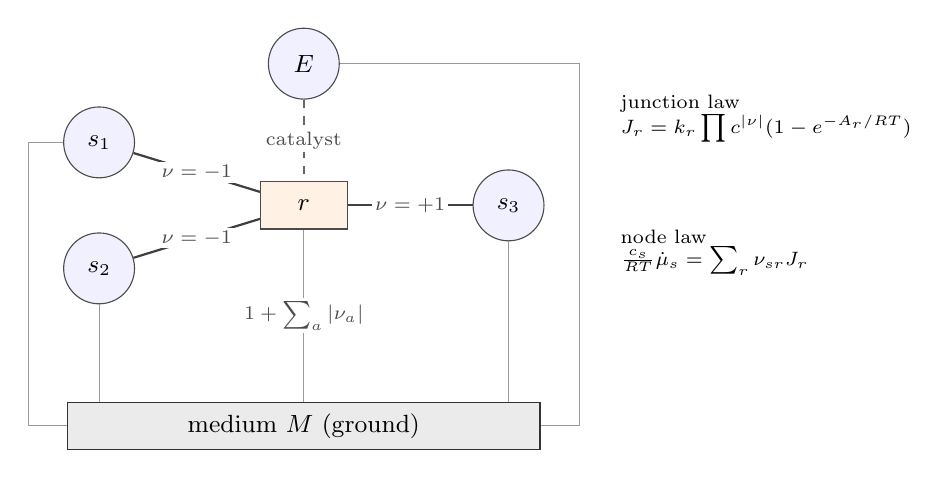
\begin{tikzpicture}[
  sp/.style={circle,draw=black!70,fill=blue!6,minimum size=9mm,inner sep=0pt,font=\small},
  jn/.style={rectangle,draw=black!70,fill=orange!10,minimum width=11mm,minimum height=6mm,font=\small},
  md/.style={rectangle,draw=black!80,fill=black!8,minimum width=60mm,minimum height=6mm,font=\small},
  st/.style={-,thick,black!75},
  mo/.style={-,thick,dashed,black!60},
  me/.style={-,thin,black!40},
  lab/.style={font=\scriptsize,black!70,fill=white,inner sep=1pt}
]
\node[sp] (s1) at (0,1.6) {$s_1$};
\node[sp] (s2) at (0,0) {$s_2$};
\node[jn] (r) at (2.6,0.8) {$r$};
\node[sp] (s3) at (5.2,0.8) {$s_3$};
\node[sp] (e) at (2.6,2.6) {$E$};
\node[md] (M) at (2.6,-2.0) {medium $M$ (ground)};
\draw[st] (s1) -- node[lab]{$\nu=-1$} (r);
\draw[st] (s2) -- node[lab]{$\nu=-1$} (r);
\draw[st] (r) -- node[lab]{$\nu=+1$} (s3);
\draw[mo] (e) -- node[lab]{catalyst} (r);
\draw[me] (s1.west) -- (-0.9,1.6) |- (M.west);
\draw[me] (s2) -- (s2 |- M.north);
\draw[me] (r) -- node[lab]{$1+\sum_{a}|\nu_{a}|$} (r |- M.north);
\draw[me] (s3) -- (s3 |- M.north);
\draw[me] (e.east) -- (6.1,2.6) |- (M.east);
\node[font=\scriptsize,align=left,anchor=west] at (6.5,1.9) {junction law\\$J_r = k_r\prod c^{|\nu|}(1-e^{-A_r/RT})$};
\node[font=\scriptsize,align=left,anchor=west] at (6.5,0.2) {node law\\$\frac{c_s}{RT}\dot\mu_s=\sum_r\nu_{sr}J_r$};
\end{tikzpicture}
\caption{Elements of a circuit knowledge graph.
Species (circles) carry potentials, junctions (rectangle) carry affinity and flux, and the medium $M$ is ground.
Solid edges are stoichiometric contacts with signed coefficients, the dashed edge is a modifier contact, and thin edges connect every item to the medium.
Ambient cofactors (water, the proton, orthophosphate and eleven others; \cref{sec:medium-ground}) are folded into $M$, which raises the weight of the junction's medium edge.}
\label{fig:schema}
\end{figure}

\subsection{The medium as ground}
\label{sec:medium-ground}

Fourteen small molecules are declared ambient.
They are water, the proton, orthophosphate, pyrophosphate, carbon dioxide, dioxygen and coenzyme~A.
They also include adenosine triphosphate (ATP), adenosine diphosphate (ADP) and adenosine monophosphate (AMP).
The last four are nicotinamide adenine dinucleotide (NAD) as NAD$^+$ and reduced NAD (NADH), and NAD phosphate (NADP) as NADP$^+$ and reduced NADP (NADPH).
Their potentials are taken as fixed by the cytosol, so they are not items; they are folded into $M$ (convention \conv{ambient-reservoir}).
The list is a declaration, not a finding.
Changing the list changes every downstream number, which is why the list is part of the stage digest (\cref{sec:digests}).
Every item has an edge to $M$ (convention \conv{medium-floor}), so every item is connected to ground and every separation cost of \cref{sec:cuts} is finite and positive.

\subsection{Structure without parameters}
\label{sec:structure}

Let $N$ be the stoichiometric matrix restricted to the internal species, with one column per junction.
Its rank, its left null space (conservation laws) and its right null space (steady flux modes) are properties of the system of node laws that do not depend on any rate constant.

\begin{proposition}[Blocked junctions]
\label{prop:blocked}
Hold the medium and every species not in $N$ at fixed potential.
Junction $r$ carries zero flux in every steady state of the node laws if and only if $e_r^{\top} v = 0$ for every $v\in\ker N$.
\end{proposition}
\begin{proof}
At steady state $\dot\mu_s=0$ for every internal species, so by \cref{eq:node} $NJ=0$, i.e.\ $J\in\ker N$.
If every $v\in\ker N$ has $v_r=0$, then $J_r=0$.
Conversely, if some $v\in\ker N$ has $v_r\neq0$, then $J=v$ satisfies the steady-state balance with $J_r\neq0$.
\end{proof}

In practice, an orthonormal basis $V_0$ of $\ker N$ is taken from a singular value decomposition, and $r$ is blocked when row $r$ of $V_0$ has norm below $10^{-8}$.
The numerical rank is cut at a relative singular value of $10^{-9}$.
The cut is rejected unless it falls inside a spectral gap: if the largest dropped singular value exceeds $10^{-12}$ of the largest and the smallest kept one is below $10^{-6}$ of it, the computation stops with an error.
A size-scaled cut (the common default $\epsilon\max(m,n)\sigma_1$) fell above the smallest genuine singular value of the enzyme-expanded matrix and invented null vectors; the gap rule exists because of that failure, and a regression test pins it.

\subsection{Verdicts}
\label{sec:verdicts}

\begin{definition}[Verdict]
\label{def:verdict}
A verdict is a tuple $(\ell, p, b, \rho, \delta, g)$ of a label $\ell$, a payload $p$, a blocker $b$, a remedy $\rho$, a detail record $\delta$ and an optional gate letter $g$.
The label takes one of seven values.
The label \vd{answered} means a payload is present, and \vd{certified-empty} that the question is well posed and its answer is empty.
The label \vd{absent} means a required datum is absent.
The label \vd{underdetermined} means several readings are admissible and no rule selects one.
The label \vd{undecidable} means the data cannot resolve the answer within tolerance.
The label \vd{refused} means the question is outside what the graph can state, and \vd{subfloor} that a composite power is below its declared target.
\end{definition}

Two invariants are enforced at construction time, so a verdict that violates them cannot exist:
\begin{enumerate}[label=(V\arabic*),itemsep=1pt]
  \item if $\ell\neq\vd{answered}$ then $p$ is empty;
  \item if $\ell\notin\{\vd{answered},\vd{certified-empty}\}$ then $b$ is non-empty.
\end{enumerate}
(V1) prevents a missing value from travelling downstream disguised as a number.
(V2) makes every non-answer actionable, because its blocker says what is missing and its remedy, when present, says what would supply it.
A gate letter (\cref{sec:gates}) may be attached only to \vd{certified-empty} or \vd{absent} verdicts.

The labels refine the third value of strong Kleene logic by cause \citep{kleene1952introduction}.
\vd{absent} and \vd{undecidable} both leave the answer open, but they ask for different remedies.
The first needs a new measurement; the second needs a more precise one.
A \vd{certified-empty} verdict closes the question: a completion search that finds no route has answered it.
A \vd{refused} verdict is not a failure of data at all: TECRDB states only small-molecule reactions, so asking it for the $\DG$ of a reaction with a protein participant is outside its scope.

\subsection{Provenance}
\label{sec:provenance}

\subsubsection{Basis}
\label{sec:basis}

Every value carries a basis tag: \emph{stated} (the source record asserts it), \emph{supplied} (a named convention produced it) or \emph{derived} (the kernel computed it from other values).
A fourth tag, \emph{estimated}, marks a value a model predicted, for instance by component contribution \citep{noor2013component} or as a learned turnover number \citep{li2022dlkcat}.
A fifth tag, \emph{absent}, marks a value that neither source nor convention determines.
A supplied value must name its convention; an absent value carries none.

\begin{proposition}[Basis is never laundered]
\label{prop:basis}
Order the bases \emph{stated} $<$ \emph{supplied} $<$ \emph{derived} $<$ \emph{estimated}, and let the composition of tags be their maximum, with \emph{absent} absorbing.
Then the composition is associative, commutative and idempotent, and no value computed from an estimated or derived input can carry a lower basis.
\end{proposition}
\begin{proof}
The maximum over a total order is a join on a chain, hence a semilattice operation; adjoining an absorbing element preserves associativity, commutativity and idempotence.
Monotonicity of the maximum gives the second statement.
\end{proof}

Of the 201 reactions with a chemical-reference $\DG$ (\cref{sec:res-thermo}), 75 direction verdicts are \emph{supplied} (a measured value judged under the supplied medium window) and 126 are \emph{derived}; none can be reported as stated.

\subsubsection{Gate letters for empty answers}
\label{sec:gates}

An empty or absent answer can be empty for different reasons, and the reasons matter for what to do next.
Each such verdict carries one of five letters.
The letter $+$ means witnessed absent: the source covers the case and records nothing.
The letter $-$ means not recorded: the source does not cover it, and \textsf{a} means both.
\textsf{open} means a name the source never uses, so the question cannot be put to it, and \textsf{?} means undecided.
The letter is assigned from the blocker by a fixed rule table; a \vd{certified-empty} answer defaults to $+$ because it completed and found nothing.
For example, ``no TECRDB measurement of this reaction'' is $-$, while ``participant without an identifier of the Kyoto Encyclopedia of Genes and Genomes (KEGG)'' is \textsf{open}.
The second can be closed by a cross-reference, the first only by a measurement (\cref{sec:res-db}).

\subsubsection{Ground verdicts}
\label{sec:ground}

Each fact family is generated by a typed activity that used other records, forming a provenance chain in the sense of PROV-O \citep{lebo2013provo}.
Walking the chain backwards, three bits are collected: $g$ (a generation is recorded), $c$ (a contact activity, i.e.\ a measurement of the object, is reachable) and $d$ (a derivation is reachable).
The ground verdict is
\begin{center}
\begin{tabular}{@{}cccl@{}}
\toprule
$g$ & $c$ & $d$ & ground verdict \\
\midrule
0 & 0 & 0 & symbol (nothing generated it) \\
1 & 0 & 0 & collapsed (curation with no contact) \\
1 & 1 & 0 & index (a measurement of the object) \\
1 & 0 & 1 & icon (a model of the object) \\
1 & 1 & 1 & composite (measurement and derivation) \\
\bottomrule
\end{tabular}
\end{center}
with an override: if any model prediction (component contribution, machine-learned prediction, group contribution) is reachable, the verdict is \emph{estimated}.
The terms follow Peirce's division of signs by their relation to their object \citep{peirce1932collected}: an index is physically connected to its object, an icon resembles it, a symbol relates to it by convention only.
Over the kernel's fact families, TECRDB rows, SABIO-RK parameters, PaxDb abundances and Protein Data Bank coordinates are indices.
Every pooled or derived $\DG$, every direction verdict, every retention factor and every distance measured on a crystal structure is composite.
AlphaFold models, and the contact graphs and enzyme cycles built on them, are icons.
Reactome stoichiometry, UniProt Enzyme Commission (EC) numbers and eQuilibrator microspecies tables are collapsed.
The chemical potential $\mu$, which is never stored, is a symbol.

\subsubsection{Stage digests}
\label{sec:digests}

A derived value is valid only for the content and conventions it was computed on.
Each stage records a digest: the SHA-256 of each input file, the SHA-256 of the canonical serialisation of its conventions, and the SHA-256 of both together.
A stage is current if recomputing the digest reproduces it.
Changing the pH window makes the medium stage stale; the check is discriminating because its control (an unchanged window) stays current.

\subsubsection{Check markers}
\label{sec:checks}

A check is reported as \emph{pass}, \emph{fail}, \emph{non-discriminating} or \emph{uncontrolled}.
It is non-discriminating when its control passes as well: a test that cannot fail tells nothing.
Every test in the kernel's suite (\cref{app:tests}) has a control that must change the outcome.

\subsection{Counted weights and separation costs}
\label{sec:cuts}

All edge weights used for cuts are counts: stoichiometric coefficients, heavy-atom contacts, exposed atoms.
Real-valued quantities such as Gibbs energies or conductances stay in the element laws and never become cut weights.

\begin{definition}[Local cut key]
\label{def:cutkey}
Let $H=G-M$ be the item graph and $B_r(v)$ the ball of radius $r$ about item $v$ in $H$.
Build a flow network on $B_r(v)$ with the edge weights of $G$ as capacities, and join every edge from $B_r(v)$ to a vertex outside it (including $M$) to a single sink $T$.
The \emph{local separation cost} $\sigma_r(v)$ is the maximum flow from $v$ to $T$, equal to the minimum cut \citep{ford1956maximal}.
Write $\delta_r(v)$ for the size of the source side of the minimal minimum cut, $\beta_r(v)$ for the smallest edge weight inside the ball or on its medium edges, and $\pi_r(v)=1-\beta_r(v)/\sigma_r(v)$ for the derived power.
The cut key of $v$ is $(\sigma_r,\delta_r)$.
\end{definition}

Maximum flows are computed by preflow--push \citep{goldberg1988preflow}; the source side of the minimal cut is the set reachable from $v$ in the residual network.
The \emph{global separation cost} $\sigma(v)$ is the maximum flow from $v$ to $M$ in the connected component of $v$.

\begin{proposition}[Expansion never lowers separation cost]
\label{prop:monotone}
Let $G'$ be obtained from $G$ by adding vertices and edges with non-negative weights, without changing any existing weight.
Then $\sigma_{G'}(v)\ge\sigma_G(v)$ for every vertex $v$ of $G$.
\end{proposition}
\begin{proof}
Let $(X',\bar X')$ be a minimum $v$--$M$ cut in $G'$ and $X=X'\cap V(G)$.
Every edge of $G$ crossing $(X,V(G)\setminus X)$ also crosses $(X',\bar X')$ in $G'$ with the same weight, so the cut value of $X$ in $G$ is at most that of $X'$ in $G'$.
Hence $\sigma_G(v)\le\sigma_{G'}(v)$.
\end{proof}

The proposition is why proteins are attached to the graph by expansion (\cref{sec:attach}): new residue vertices and edges only.
It does not cover the tempting alternative of replacing an existing counted weight by a real-valued one, and \cref{sec:res-proteins} shows that this alternative does lower separation costs.

\paragraph{Colour refinement.}
Classes of structurally equivalent items are computed by colour refinement \citep{weisfeiler1968reduction}.
The initial colour of an item is (kind, $\sigma_1$, $\delta_1$); each round replaces the colour by the pair (colour, sorted multiset of (edge role, edge weight, neighbour colour)).
Labels are canonical: colours are ranks of sorted signatures.

\begin{proposition}[Refinement is invariant and monotone]
\label{prop:refine}
The final partition is invariant under any relabelling of the items, and the partition after each round refines the one before.
\end{proposition}
\begin{proof}
Every quantity entering a colour is a function of the weighted, role-labelled graph alone, and canonical ranking removes any dependence on item names; hence an isomorphism maps classes to classes.
The new colour contains the old colour as a component, so two items with different old colours have different new colours.
\end{proof}

Refinement stops when the number of classes no longer grows.
Items left in a shared class cannot be separated by any number of further rounds, just as two analytes of equal retention cannot be separated by any column length \citep{giddings1991unified}.
The information still needed to locate an item within its class is $\log_2 s$ bits for a class of size $s$.
With $n_c$ distinct values of the initial key, at least $\log K/\log n_c$ independent keys are needed to give $K$ items distinct positions.

\subsection{Ladders}
\label{sec:ladders}

A series chain reservoir $\to r_1\to s_1\to\cdots\to r_n\to s_n\to M$ in the linear tangent $J=GA$ has resistances $R_k=1/G_k$ and a medium exchange resistance $R_M$.
Define the power of rung $k$ as the fraction of the remaining drop it closes:
\begin{equation}
  \pi_k = \frac{R_k}{R_k+R_{k+1}+\cdots+R_n+R_M}.
\end{equation}

\begin{proposition}[Ladder powers telescope]
\label{prop:ladder}
With $R_{\mathrm{tot}}=\sum_k R_k + R_M$, the composite power is $1-\prod_k(1-\pi_k) = 1-R_M/R_{\mathrm{tot}}$, and the share $R_k/R_{\mathrm{tot}}$ of rung $k$ equals its flux control coefficient $\partial\ln J/\partial\ln G_k$.
\end{proposition}
\begin{proof}
$1-\pi_k=(R_{k+1}+\cdots+R_M)/(R_k+\cdots+R_M)$, so the product telescopes to $R_M/R_{\mathrm{tot}}$.
For the share, $J=\Delta A/R_{\mathrm{tot}}$, hence $\partial\ln J/\partial\ln G_k = -\partial\ln J/\partial\ln R_k = R_k/R_{\mathrm{tot}}$, the flux control coefficient of metabolic control analysis \citep{kacser1973control,heinrich1974linear}.
\end{proof}

A ladder's rung powers are therefore derived from the circuit once conductances exist, and \vd{absent} until then.
A declared target for the composite power that the ladder does not reach yields \vd{subfloor}, with the shortfall in the verdict.
